
\begin{figure}[t]
\centering
\subfloat[Without NoC.]{
   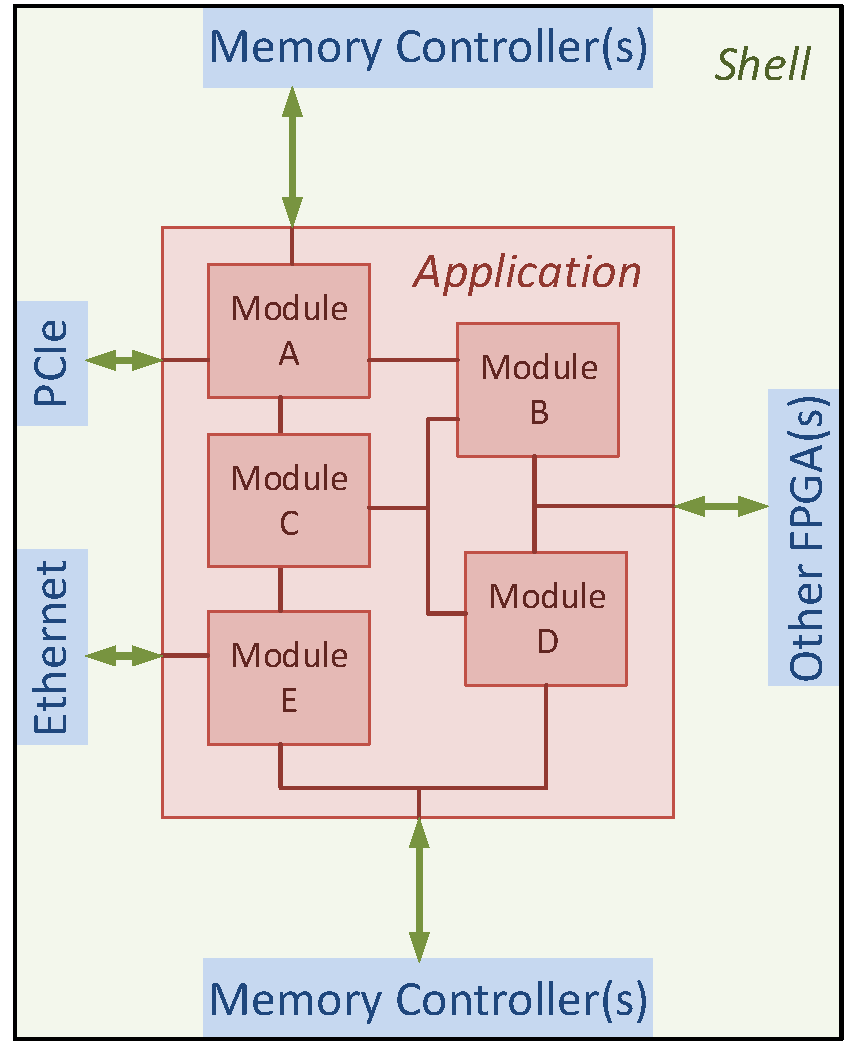
\includegraphics[width=0.5\columnwidth,keepaspectratio]{images/computing}
   \label{computing_no_noc}
 }
\subfloat[With NoC]{
   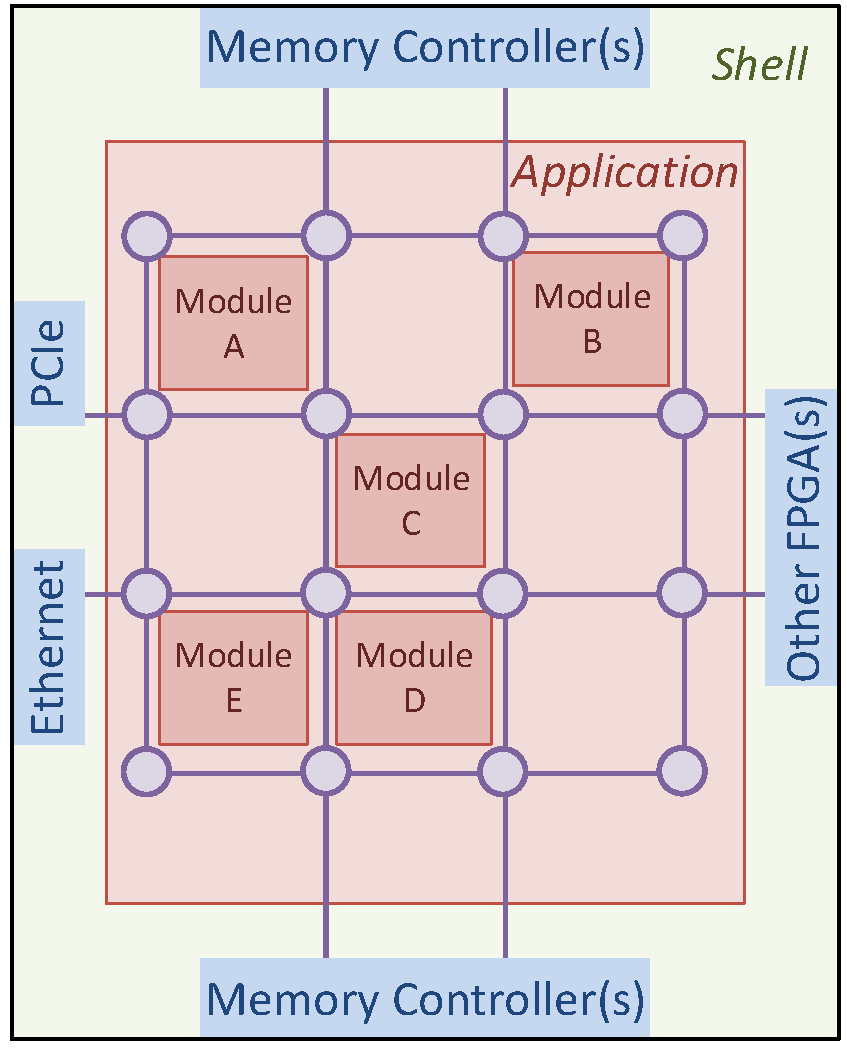
\includegraphics[width=0.5\columnwidth,keepaspectratio]{images/computing_w_noc}
   \label{computing_w_noc}
 }
\caption{A sample FPGA compute accelerator consists of a shell and the application logic.}
\label{computing}
\end{figure}

In this future-looking section, we discuss how an embedded NoC could improve FPGA compute acceleration such as that with data center computing~\cite{Putnam2014} or the OpenCL compute model~\cite{opencl}.
FPGA accelerators consist primarily of two components; the application logic itself, and the \textit{shell} which implements the communication infrastructure for the application.
Fig.~\ref{computing} illustrates the implementation of a compute accelerator, both with and without an embedded NoC.

As Fig.~\ref{computing} shows, a shell consists primarily of a system-level interconnect that connects an application to the host CPU, I/O and memory interfaces, and other FPGAs~\cite{Putnam2014,opencl}.
Built out of soft buses, Microsoft's implementation of this shell occupies approximately one quarter (23\% area) of a large Stratix~V FPGA device~\cite{Putnam2014}.
We believe this area overhead can be reduced if an NoC (with an area of \til1.3\%) is leveraged to interconnect modules in the shell and accelerator -- previous work has already shown that an NoC uses less area and power than soft buses when connecting a system to DDRx memory~\cite{micro}.
Besides the area overhead, it is challenging to meet the timing constraints of the many fast I/O interfaces to which the shell connects -- designers would typically \textit{lock down} the placement and routing of the shell once timing closure is attained, and present standard fixed-location interfaces to the FPGA application logic~\cite{Putnam2014}.
Conversely, an NoC with direct IOLinks to external interfaces can significantly ease timing closure.
Furthermore, any NoC router can be used to connect application modules to the shell instead of fixed-location interfaces -- this would relax the placement and routing constraints of the application and likely improve its performance.
As the JPEG application case study showed, overall application frequency can also be much more predictable with an NoC.
This predictability is especially important when high-level languages (such as OpenCL) are used, and the designer has no direct way to improve operating frequency.

In such compute accelerators, partial reconfiguration is quickly becoming an important feature~\cite{Putnam2014}.
Using partial reconfiguration, the application could either be repaired or replaced without powering down the FPGA, or the data center in which it lies.
To successfully connect a partially reconfigured module, current accelerator shells must provide fixed interfaces and interconnect to the \textit{superset} of the modules that could be partially reconfigured on the FPGA.
This method could be wasteful and complex, and it is often difficult to predict exactly what will be reconfigured in the future.
Instead, we propose using the NoC FabricPorts as a standard, yet flexible interface to partially reconfigured modules.
This avoids the need to explicitly provision a soft bus interface and interconnect for all partially reconfigured modules, since any module connected through a FabricPort will be able to communicate with the rest of the application and I/Os through the embedded NoC.
Our packet processor, NoC-PP in Section~\ref{sec_pp}, could benefit from partial reconfiguration -- the processing modules can be partially reconfigured to update or change the networking protocol.



%\hl{shell construction and using IOLinks to more easily create portable and compatible shells (communication infrastructure).}

%\hl{high-level languages focus on kernels which are then interconnected through a pre-existing NoC. Implementation of things like OpenCL channels. More predictable frequency a big plus for these systems in which the software programmer has no notion of critical path or timing when using the high-level tools}

%\hl{partial reconfiguration in which the NoC can provide a standard interface to which partially-reconfigured modules connect.}
